
\section{Background}
\label{sec:ncdn-background}

\subsection{NCDN architecture} 

A typical \ncp\ architecture, as shown in Figure \ref{fig:NCDNArch}, resembles the architecture of a global CDN but with some important differences. First,  the content servers are deployed at points-of-presence (PoPs) within the network rather than globally across the Internet as the \ncp\ is primarily interested in optimizing content delivery for its own customers and end-users. Second, and more importantly, the NCDN owns and manages the content servers as well as the underlying network. Content providers that purchase content delivery service from the \ncp\ publish their content to origin servers that they maintain external to the \ncp\ itself. 

Each PoP is associated with a distinct set of end-users who request content such as web, video, downloads etc.  An end-user's request is first routed to the content servers at the PoP to which the end-user is connected.  If a content server at that PoP has the requested content in their cache, it serves that to the end-user. Otherwise, if the requested content is cached at other PoPs, the content is downloaded from a nearby PoP and served to the end-user. If the content is not cached in any PoP, it is downloaded directly from  the content provider's origin servers.

\begin{figure}[t]
\centerline{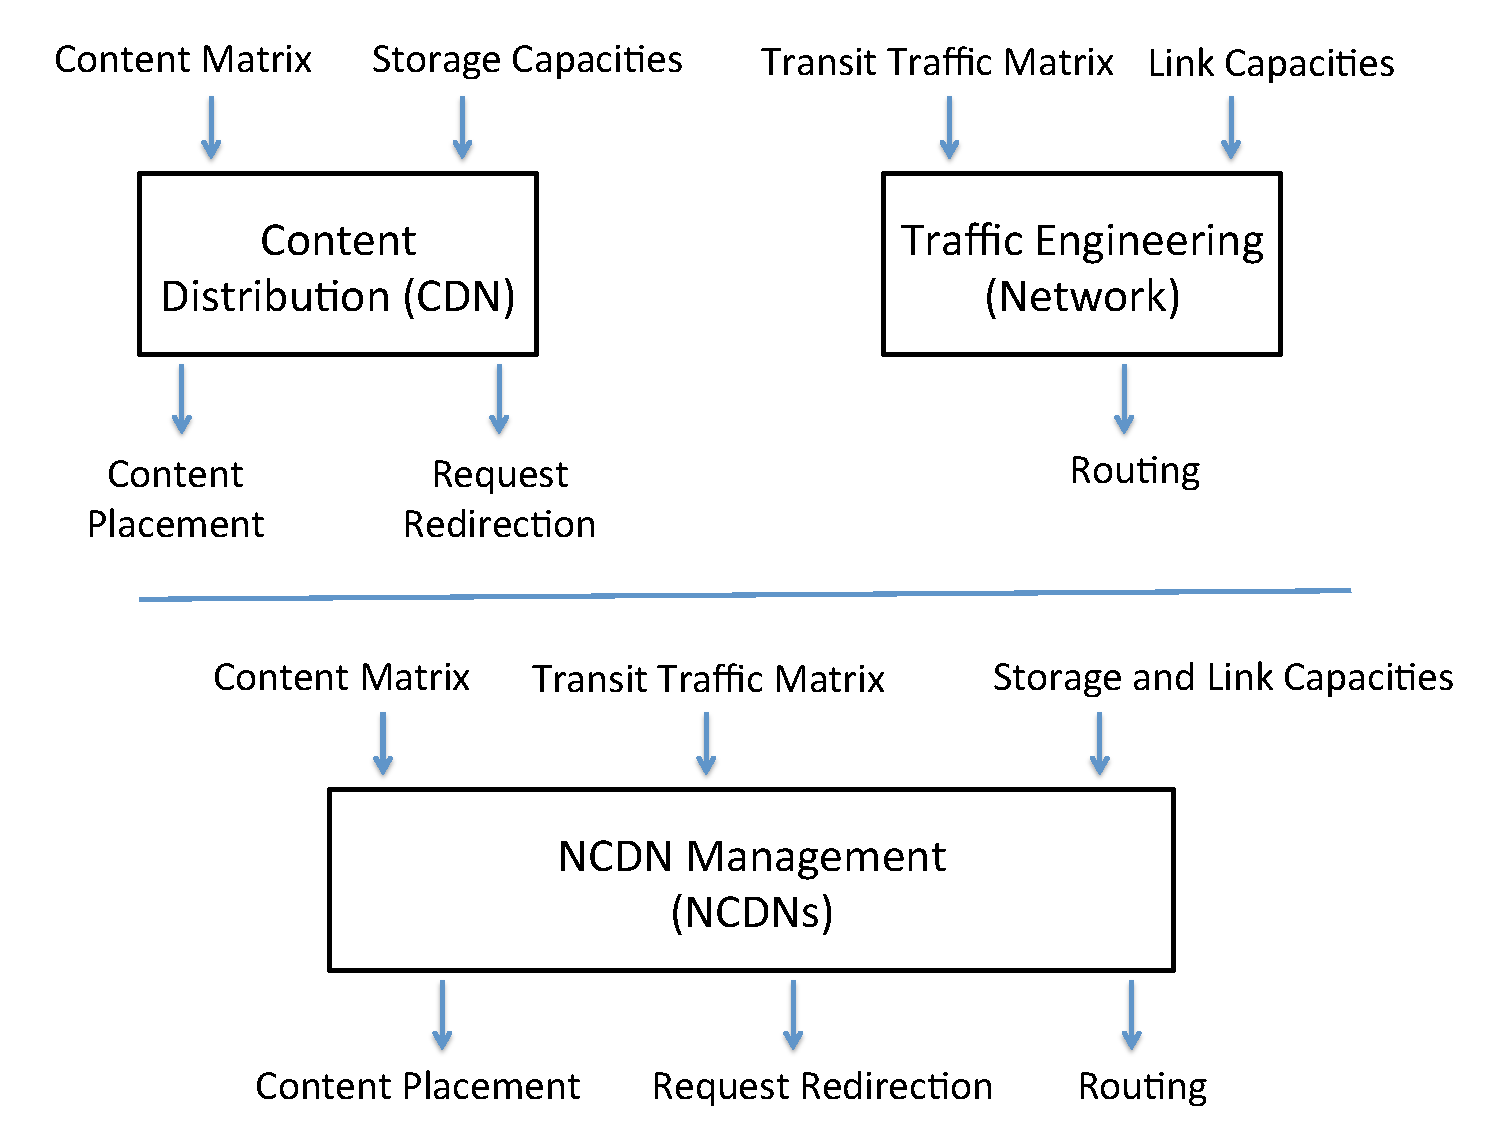
\includegraphics[scale=0.31]{ncdnpaper/NCDN}}
\caption{(Top) Traditional formulation with content delivery and traffic engineering optimized separately. (Bottom) Our new formulation of NCDN magamenent as a joint optimization.}
\vspace{-0.2in}
\label{fig:ncdntraditional}
\end{figure}

\subsection{NCDN management objectives and schemes}

Managing content delivery as well as the underlying network makes the costs and objectives of interest to an \ncp\ different from that of a traditional CDN or a traditional ISP. Figure \ref{fig:ncdntraditional} (top) shows the traditional concerns of content delivery and traffic engineering as addressed by a traditional CDN and a traditional ISP respectively, while Figure \ref{fig:ncdntraditional} (bottom) shows the combined concerns that an NCDN must address. 

NCDN management refers to the combined task content delivery and traffic engineering performed by an NCDN. We classify the possible NCDN mangement schemes into two axes as discussed below.

\textbf{Demand-aware vs. demand-oblivious:} We summarize pros and cons of demand-aware and demand-oblivious approaches for content delivery and ISP traffic engineering discussed in Chapter \ref{ch:te-background}. A demand-aware approach for ISP traffic engineering, which periodically computes and updates routing based on traffic matrices, has been shown to be superior to a demand-oblivous approach that configures routes statically. A demand-oblivious approach is more common for content delivery, in which content placement and request redirection is done using a simple online algorithm such as LRU cache replacement for content placement. In comparison, a demand-aware approach is more complex as it requires network-wide measurement of content-level demand and is potentially computationally expensive, but it could yield benefits for some workloads \cite{Applegate2010}.

\textbf{Independent vs. joint optimization:} Unlike a traditional ISP or a traditional NCDN, an NCDN controls placement, redirection and routing on its network. An NCDN may simply treat placement, redirection and routing independently, or it may seek to jointly optimize these decisions to leverage the interaction between them. 
The example in Chapter \ref{ch:te-background}, Section \ref{sec:bg-ncdn} illustrates the interaction between placement and routing in an NCDN. A joint-optimization approach may potentially yield benefits, as has been demonstrated in a different scenario where two distint entities ISPs and content providers jointly optimize their network routing and request redirection. Developing a joint optimization for NCDN and evaluating its benefits over independent optimization of placement, redirection and routing are among the key goals of our work.

% As \ncp s own and manage the infrastructure for content delivery as well as the underlying network, they are in a powerful position to control all three of placement, routing, and redirection.

%As \ncp s own and manage the infrastructure for content delivery as well as the underlying network, they are in a powerful position to control all three of placement, routing, and redirection (Figure \ref{fig:ncdntraditional}). In particular, \ancp\ can place content in a manner that ``shapes'' the traffic demands so as to jointly optimize both user-perceived latency as well as network cost.
